\section{Method}
\label{sec:metodo}

Figure~\ref{fig:flujo} summarises the pipeline: tasks are rated by models, consensus is taken across models, consensus is weighted into occupations, occupations are weighted into countries, and every step is validated or bootstrapped.
The design was preregistered on the Open Science Framework before the first model call, with an embargo until January 2027; the hypotheses, the rubric hash and the sample seeds are in the registration and in \texttt{docs/OSF\_PREREGISTRO\_EN.md}.

\begin{figure}[t]
  \centering
  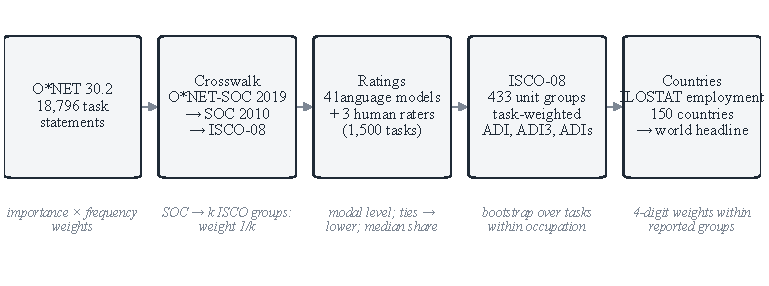
\includegraphics[width=\linewidth]{fig/fig2_flujo}
  \caption{From task statements to a country atlas. Inputs on the left, validation steps below the main flow. Figure generated by \texttt{figuras/fig2\_flujo.py}.}
  \label{fig:flujo}
\end{figure}

\subsection{Rubric}

Each task is rated with the rubric reproduced in Appendix~\ref{app:rubrica}.
The prompt contains the reference technology, the four level definitions, the occupation title and the task text, and asks for a single JSON object with eight fields: level (0--3), share of the task's working time an agent could take over (0--100), minutes a competent human needs for one instance, four barrier flags (physical, accountability, trust, access) and a confidence label.
The rubric contains no example tasks, so no task in the data can anchor the rating of another.
The file was frozen at registration; its SHA-256 hash is \texttt{bcd076fb\ldots0ea0e46} (full value in Appendix~\ref{app:rubrica}), and the scoring script refuses to run the main pass unless the file on disk matches it.
A pilot of at most 300 tasks (seed 20261020) checked JSON compliance and cost; pilot ratings are discarded.

\subsection{Raters: language models}

Models are queried one task per call, with no other task or rating in context, through the Claude Code command-line interface (\texttt{claude -p --output-format json}) rather than through a raw API.
The primary rater is Claude Sonnet and the secondary rater is Claude Haiku; Claude Opus is run as an optional third rater on the full task set if budget allows and otherwise on the validation sample.
Every call is logged with the interface version, the model identifier returned by the interface, the prompt hash, the duration and the outcome in \texttt{docs/llm-llamadas.jsonl}, which doubles as the manuscript's declaration of AI use.
The interface does not expose a temperature setting, so the ratings are not deterministic by construction.
We therefore measure stability directly: a random subsample of \cifra{n.testretest} tasks is rated a second time by each model under identical prompts, and we report exact agreement and quadratic-weighted kappa between the two passes (Sonnet: \cifra{agree.testretest.sonnet.kappa}; Haiku: \cifra{agree.testretest.haiku.kappa}).
% and in the deviations appendix before submission. The sentence below assumes that entry exists.
Two of the four raters are open-weights models queried through their providers' APIs at temperature zero (DeepSeek V4-Pro and Kimi K2.6); the two Claude models are queried through the Claude command-line interface, which does not expose temperature. Exact model identifiers and the interface version are recorded in \texttt{docs/MODELOS.md} before the main run.
Calls whose output fails validation (malformed JSON, a level outside 0--3, a share outside 0--100) are retried up to five times; tasks that still fail are excluded for that model only, and the counts are reported (\cifra{n.fallos.sonnet} for Sonnet, \cifra{n.fallos.haiku} for Haiku).

\subsection{Aggregation}

Let $t$ index tasks, $m$ models, $o$ ISCO-08 unit groups and $c$ countries.
The consensus level of a task is the modal level across models, with ties resolved to the lower level; the consensus share is the median share across models.
Task weights $w_{ot}$ are importance times mean frequency, normalised within the O*NET occupation, multiplied by the crosswalk weight ($1/k$ for a SOC code that maps to $k$ ISCO groups) and renormalised so that $\sum_t w_{ot} = 1$ within each unit group.
The primary occupation index is the share of task weight at partial delegation or above:
\begin{equation}
  \mathrm{ADI}_o = \sum_{t} w_{ot}\, \mathbf{1}[\mathrm{level}_t \geq 2],
  \label{eq:adi_o}
\end{equation}
with two preregistered variants, the share at full delegation and the expected share of working time delegable:
\begin{equation}
  \mathrm{ADI3}_o = \sum_{t} w_{ot}\, \mathbf{1}[\mathrm{level}_t = 3], \qquad
  \mathrm{ADIs}_o = \sum_{t} w_{ot}\, \frac{\mathrm{share}_t}{100}.
  \label{eq:adi_var}
\end{equation}
The country index is the employment-weighted mean over the occupational groups $g$ the country reports:
\begin{equation}
  \mathrm{ADI}_c = \frac{\sum_{g} e_{cg}\, \mathrm{ADI}_g}{\sum_{g} e_{cg}},
  \label{eq:adi_c}
\end{equation}
where $e_{cg}$ is ILOSTAT employment and $g$ runs over two-digit sub-major groups if the country reports them for a year from 2019 onward and over one-digit major groups otherwise.
Within a reported group, unit-group indices are averaged with employment weights pooled from the countries in the same World Bank income group that report finer detail; equal weights within the group are the preregistered sensitivity check.
The world headline is the employment-weighted mean of $\mathrm{ADI}_c$ over the 151 included countries, and the income-group figures are the same mean within each group.

\subsection{Human validation}

Three raters with at least a university degree in economics, engineering or social science rate 1,500 tasks each.
The sample is stratified by ISCO-08 major group in proportion to world employment, with a minimum of 60 tasks per group (\texttt{validacion/muestra.py}, seed 20261020); each rater receives the same tasks in an independent random order (seeds 20261021--20261023) in a spreadsheet that contains the rubric and no model output.
Raters are blind to the models and to each other, are trained on 20 practice tasks outside the sample, and are asked not to use AI tools while rating.
We report quadratic-weighted kappa \citep{cohen1968weighted} for each pair of raters and Krippendorff's alpha for ordinal data \citep{krippendorff2004reliability} among the three humans (\cifra{agree.alpha.humano}; pairwise $\kappa$ from \cifra{agree.kappa.humano.min} to \cifra{agree.kappa.humano.max}) and between the human majority and the model consensus (\cifra{agree.alpha.humano.modelo}; $\kappa$ = \cifra{agree.kappa.humano.modelo}).
The preregistered acceptance threshold for the primary rater is $\alpha \geq 0.60$; results are reported whatever the value.
The 1,500 tasks give a 95\% confidence-interval half-width below 0.03 for an alpha near 0.60.

\subsection{Convergent validity}

Hypothesis H3 states that occupation-level ADI correlates positively with the exposure scores of \citet{eloundou2024gpts} and the AIOE of \citet{felten2021occupational}, with Pearson $r$ between 0.40 and 0.80 for each: above 0.80 would mean ADI adds little beyond exposure, below 0.40 would question its validity.
Both comparison indices are carried to ISCO-08 with the bridge of Section~\ref{sec:datos}.
We report Pearson and Spearman coefficients (Eloundou: $r$ = \cifra{h3.r.eloundou}, $\rho$ = \cifra{h3.rho.eloundou}; Felten: $r$ = \cifra{h3.r.felten}, $\rho$ = \cifra{h3.rho.felten}), and, as exploratory comparisons, the same statistics against \citet{webb2020impact}, \citet{eisfeldt2023generative}, the ILO index \citep{gmyrek2025generative} and the Agentic Adoption Index \citep{lee2026delegates}.

\subsection{Hypothesis tests}

H1, the delegation divide, is an ordinary least squares regression of $\mathrm{ADI}_c$ on log GDP per capita at purchasing power parity, and a second specification with income-group dummies with high income as reference; the test on the slope is one-sided at $\alpha$ = 0.05.
H2, the adoption gap, standardises $\mathrm{ADI}_c$ and AEI usage per working-age adult to mean zero and unit variance over the countries with both and regresses the difference on income-group dummies; the one-sided test is that the middle-income coefficients are positive.
H4, task length, is a logistic regression of full delegation on log human minutes and its square at the task level, with standard errors clustered by occupation and minutes winsorised at 1 and 4,800; the hypothesis is a positive linear and a negative quadratic coefficient.

\subsection{Inference and placebo}

Uncertainty from the rating step is propagated by a nonparametric bootstrap over tasks: 1,000 draws, tasks resampled within occupation, each draw recomputing Equations~\ref{eq:adi_o}--\ref{eq:adi_c}, the headline and the regression coefficients \citep{efron1993introduction}.
All intervals in the paper are 95\% percentile intervals from this bootstrap unless stated otherwise.
As a placebo, we shuffle task ratings across occupations 1,000 times, holding each occupation's task count and weights fixed, and recompute the occupational index; the observed dispersion of $\mathrm{ADI}_o$ across unit groups is compared with this null (\cifra{placebo.p}).
A rating that carried no occupation-specific information would produce occupational indices indistinguishable from the shuffled ones.
Robustness checks preregistered as exploratory are reported model by model, with ESCO skills instead of O*NET tasks, with uniform task weights, and without the seven imputed groups.
